\documentclass[11pt]{article}
\usepackage{listings}
\usepackage{tikz}
\usetikzlibrary{arrows,automata,shapes}

\newtheorem{defn}{Definition}
\newtheorem{crit}{Criterion}

\newcommand{\handout}[5]{
  \noindent
  \begin{center}
  \framebox{
    \vbox{
      \hbox to 5.78in { {\bf Software Testing, Quality Assurance and Maintenance } \hfill #2 }
      \vspace{4mm}
      \hbox to 5.78in { {\Large \hfill #5  \hfill} }
      \vspace{2mm}
      \hbox to 5.78in { {\em #3 \hfill #4} }
    }
  }
  \end{center}
  \vspace*{4mm}
}

\newcommand{\lecture}[4]{\handout{#1}{#2}{#3}{#4}{Lecture #1}}
% 1-inch margins, from fullpage.sty by H.Partl, Version 2, Dec. 15, 1988.
\topmargin 0pt
\advance \topmargin by -\headheight
\advance \topmargin by -\headsep
\textheight 8.9in
\oddsidemargin 0pt
\evensidemargin \oddsidemargin
\marginparwidth 0.5in
\textwidth 6.5in

\parindent 0in
\parskip 1.5ex
%\renewcommand{\baselinestretch}{1.25}

\begin{document}

\lecture{6 --- January 16, 2015}{Winter 2015}{Patrick Lam}{version 1}

\section*{Some binary distinctions}
Let's digress for a bit and define some older terms which we won't use much
in this course, but which we should discuss briefly.

\begin{itemize}
\item \emph{Black-box testing.} Deriving tests from external descriptions
of software: specifications, requirements, designs; anything but the code.
\item \emph{White-box testing.} Deriving tests from the source code, e.g.
branches, conditions, statements.
\end{itemize}

Our model-based approach makes this distinction less important.

\section*{Test paths and cases}

We resume our graph coverage content with the following definition:

\begin{defn}
A graph is \emph{single-entry/single-exit} (SESE) if $N_0$ and $N_f$
have exactly one element each. $N_f$ must be reachable from every node
in $N$, and no node in $N \setminus N_f$ may be reachable from $N_f$, unless $N_0
= N_f$.
\end{defn}
The graphs that we'll be talking about in this course will almost
always be SESE.

Here's another example of a graph, which happens to be SESE, and
test paths in that graph. We'll call this graph $D$, for double-diamond,
and it'll come up a few times.

\begin{center}
\label{D}
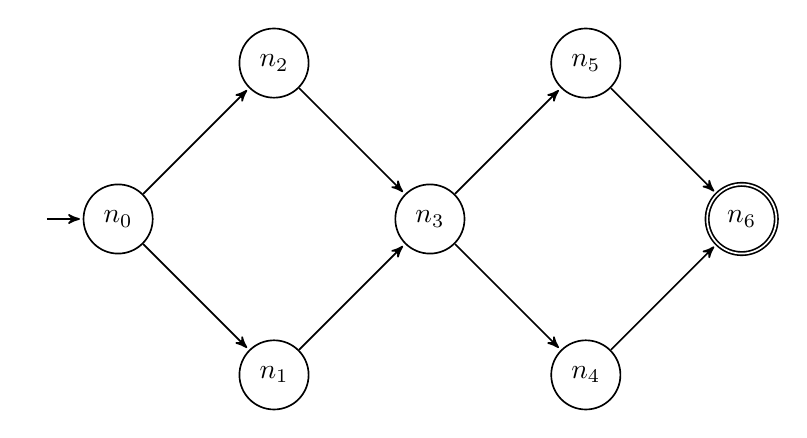
\begin{tikzpicture}[->,>=stealth',shorten >=1pt,auto,node distance=2.8cm,
                    semithick,initial text=]

  \node[initial,state]   (n0)                     {$n_0$};
  \node[state]           (n1) [below right of=n0] {$n_1$};
  \node[state]           (n2) [above right of=n0] {$n_2$};
  \node[state]           (n3) [below right of=n2] {$n_3$};
  \node[state]           (n4) [below right of=n3] {$n_4$};
  \node[state]           (n5) [above right of=n3] {$n_5$};
  \node[accepting,state] (n6) [below right of=n5] {$n_6$};
  
  \path (n0) edge              node {} (n1)
             edge              node {} (n2)
        (n1) edge              node {} (n3)
        (n2) edge              node {} (n3)
        (n3) edge              node {} (n4)
        (n3) edge              node {} (n5)
        (n4) edge              node {} (n6)
        (n5) edge              node {} (n6);
\end{tikzpicture}
\end{center}
Here are the four test paths in $D$:
\begin{eqnarray*}
&[n_0, n_1, n_3, n_4, n_6]& \\
&[n_0, n_1, n_3, n_5, n_6]& \\
&[n_0, n_2, n_3, n_4, n_6]& \\
&[n_0, n_2, n_3, n_5, n_6]&
\end{eqnarray*}

We next focus on the path $p = [n_0, n_1, n_3, n_4, n_6]$ and use it
to explain several path-related definitions. We can say that $p$
\emph{visits} node $n_3$ and edge $(n_0, n_1)$; we can write $n_3 \in
p$ and $(n_0, n_1) \in p$ respectively. 

Let $p' = [n_1, n_3, n_4]$. Then $p'$ is a \emph{subpath} of $p$.

\paragraph{Test cases and test paths.} We connect test cases and
test paths with a mapping $\mbox{path}_G$ from test cases to test
paths; e.g. $\mbox{path}_G(t)$ is the set of test paths corresponding
to test case $t$.
\begin{itemize}
\item usually we just write $\mbox{path}$ since $G$ is obvious from the context.
\item we can lift the definition of $\mbox{path}$ to test sets $T$ by defining
$\mbox{path}(T) = \{ \mbox{path}(t) | t \in T \}$.
\item each test case gives at least one test path. If the software is
  deterministic, then each test case gives exactly one test path;
  otherwise, multiple test cases may arise from one test path.
\end{itemize}

\tikzstyle{block} = [rectangle, draw, fill=blue!20, 
    text width=3em, text centered, rounded corners, minimum height=2em]

Here's an example of deterministic and nondeterministic control-flow graphs:
\begin{center}
\begin{tikzpicture}[->,>=stealth',shorten >=1pt,auto,node distance=2cm,
                    semithick,initial text=]

  \node[initial,block,text width=5em]   (A)              {\tt if (x > 3)};
  \node[block]           (T) [below right of=A] {};
  \node[block]           (F) [below left of=A] {};
  \node[accepting,block] (C) [below left of=T] {};
  
  \draw (A) -> (T) node [near end] {$x = 5$};
  \draw (A) -> (F) node [yshift=.2em, xshift=-4em,at start] {$x = 0$};
  \draw (T) -> (C);
  \draw (F) -> (C);

\end{tikzpicture}
\begin{tikzpicture}[->,>=stealth',shorten >=1pt,auto,node distance=1.5cm,
                    semithick,initial text=]

  \node[initial,block,text width=12em]   (A)              {\tt if (x.hashCode() > 3)};
  \node[block]           (T) [below right of=A] {};
  \node[block]           (F) [below left of=A] {};
  \node[accepting,block] (C) [below left of=T] {};
  
  \path (A) edge              node {} (T)
        (A) edge              node {} (F)
        (T) edge              node {} (C)
        (F) edge              node {} (C);
\end{tikzpicture}
\end{center}
Causes of nondeterminism include dependence on inputs; on the thread
scheduler; and on memory addresses, for instance as seen in calls to 
the default Java {\tt hashCode()} implementation. 

Nondeterminism makes it hard to check test case output, since more
than one output might be a valid result of a single test input.

\paragraph{Indirection.} Note that we will describe coverage criteria
with respect to \emph{test paths}, but we always run \emph{test cases}.

\newpage
\paragraph{Example.} Here is a short method, the associated control-flow
graph, and some test cases and test paths.

\begin{center}
\begin{minipage}{10em}
\vspace*{-8em}
\begin{lstlisting}
int foo(int x) {
  if (x < 5) {
    x ++;
  } else {
    x --;
  }
  return x;
}
\end{lstlisting}
\end{minipage}
\begin{tikzpicture}[->,>=stealth',shorten >=1pt,auto,node distance=2cm,
                    semithick,text width=10em,initial text=]

  \node[initial,block,text width=10em]   (A)              {\tt (1) if (x < 5)};
  \node[block,text width=6em]           (T) [below right of=A] {\tt (2) x++};
  \node[block,text width=6em]           (F) [below left of=A] {\tt (3) x--};
  \node[accepting,block,text width=10em] (C) [below left of=T] {\tt (4) return x};

  \draw (A) -> (T) node [near end] {T};
  \draw (A) -> (F) node [yshift=.2em, xshift=-2.5em,at start] {F};
  \draw (T) -> (C);
  \draw (F) -> (C);
\end{tikzpicture}
\end{center}

\begin{itemize}
\item Test case: $x = 5$; test path: $[(1), (3), (4)]$.
\item Test case: $x = 2$; test path: $[(1), (2), (4)]$.
\end{itemize}

Note that (1) we can deduce properties of the test case from the test path; and
(2) in this example, since our method is deterministic, the test case 
determines the test path.

\subsection*{Graph Coverage}
Having defined all of the graph notions we'll need for now, we apply them to
graphs. Recall our previous definition of coverage:
\begin{defn}
Given a set of test requirements \emph{TR} for a coverage criterion $C$, 
a test set $T$ \emph{satisfies} $C$ iff for every test requirement \emph{tr} in 
\emph{TR}, at least one $t$ in $T$ exists such that $t$ satisfies \emph{tr}.
\end{defn}

We apply this definition to graph coverage:
\begin{defn}
Given a set of test requirements \emph{TR} for a graph criterion $C$, 
a test set $T$ satisfies $C$ on graph $G$ iff for every test requirement
\emph{tr} in \emph{TR}, at least one test path $p$ in $\mbox{path}(T)$ 
exists such that $p$ satisfies \emph{tr}.
\end{defn}
We'll use this notion to define a number of standard testing
coverage criteria. (At this point, the textbook defines predicates, but
mostly ignores them afterwards. I'll just ignore them right away.)

Recall the double-diamond graph $D$ which we saw on page~\pageref{D}.
For the \emph{node coverage} criterion, we get the following test requirements:
\[ \{ n_0, n_1, n_2, n_3, n_4, n_5, n_6 \} \]
That is, any test set $T$ which satisfies node coverage on $D$ must include
test cases $t$; the cases $t$ give rise to test paths $\mbox{path}(t)$, and
some path must include each node from $n_0$ to $n_6$. (No single path must
include all of these nodes; the requirement applies to the set of
test paths.)

Let's formally define node coverage.
\begin{defn}
Node coverage: For each node $n \in \mbox{reach}_G(N_0)$, \emph{TR} contains
a requirement to visit node $n$.
\end{defn}

We will state all of the coverage criteria in the following form:
\begin{crit}
Node Coverage (NC): \emph{TR} contains each reachable node in $G$.
\end{crit}

We can then write
\[ \mathit{TR} = \{ n_0, n_1, n_2, n_3, n_4, n_5, n_6\}. \]

Let's consider an example of a test set which satisfies node coverage
on $D$, the double-diamond graph from last time.

Start with a test case $t_1$; assume that executing $t_1$ gives the
test path 
\[ \mbox{path}(t_1) = p_1 = [n_0, n_1, n_3, n_4, n_6].\] 
Then
test set $\{ t_1\}$ does not give node coverage on $D$, because no
test case covers node $n_2$ or $n_5$. If we can find a test case $t_2$
with test path 
\[\mbox{path}(t_2) = p_2 = [n_0, n_2, n_3, n_5, n_6],\]
then the test set $T = \{ t_1, t_2 \}$ satisfies node coverage on $D$.

{\sf What is another test set which satisfies node coverage on $D$?}\\[2em]

%We could also satisfy node coverage with test set $T'$ containing test
%cases $t_1$ and new cases $t_3$ and $t_4$ where $p_3 = [n_0, n_2, n_3,
%n_4, n_6]$ and $p_4 = [n_0, n_1, n_3, n_5, n_6]$.

Here is a more verbose definition of node coverage.

\begin{defn}
Test set $T$ satisfies \emph{node coverage} on graph $G$ if and only
if for every syntactically reachable node $n \in N$, there is some
path $p$ in $\mbox{path}(T)$ such that $p$ visits $n$.
\end{defn}

A second standard criterion is that of edge coverage.
\begin{crit}
{\bf Edge Coverage} (EC). TR contains each reachable path of length up
to 1, inclusive, in $G$.
\end{crit}
We describe edge coverage this way so that, as far as possible, new
criteria in a series will subsume previous criteria.

{\sf Here are some examples of paths of length $\le 1$:}\\[1em]
%\[ [n_3]; \qquad [n_4, n_6]. \]
Note that since we're not talking about \emph{test paths}, these
reachable paths need not start in $N_0$.

In general, paths of length $\le 1$ consist of nodes and edges. {\sf (Why not just
say edges?)}\\[3em]

%Consider this graph:
%\begin{center}
%\begin{tikzpicture}...
%\node[state,initial,accepting] (A) {};
%\end{tikzpicture}
%\end{center}
Saying ``edges'' on the above graph would not be the same as saying ``paths
of length $\le 1$''.

\newpage
Here is a more involved example:

\tikzstyle{block} = [rectangle, draw, fill=blue!20, 
    text width=3em, text centered, rounded corners, minimum height=2em]

\begin{center}
\begin{tikzpicture}[->,>=stealth',shorten >=1pt,auto,node distance=2.5cm,
                    semithick,initial text=]

  \node[initial,block]   (A)              {$n_0$};
  \node[block]           (B) [below right of=A] {$n_1$};
  \node[accepting,block] (C) [below left of=B] {$n_2$};
  
  \path (A) edge              node[right] {$x < y$} (B)
        (A) edge              node[left] {$x \ge y$} (C)
        (B) edge              node {} (C);
\end{tikzpicture}
\end{center}

Let's define
\begin{eqnarray*}
\mbox{path}(t_1) &=& [n_0, n_1, n_2] \\
\mbox{path}(t_2) &=& [n_0, n_2] 
\end{eqnarray*}

Then 
\begin{eqnarray*}
T_1 &=& \hspace*{5em} \mbox{\sf satisfies node coverage}\\
T_2 &=& \hspace*{5em} \mbox{\sf satisfies edge coverage}
\end{eqnarray*}

\paragraph{Going beyond 1.} So far we've seen length $\le 0$ (node coverage)
and length $\le 1$. Of course, we can go to lengths $\le 2$, etc., but
we quickly get diminishing returns. Here is the criterion for length $\le 2$.

\begin{crit}
{\bf Edge-Pair Coverage.} (EPC) TR contains each reachable path of length
up to 2, inclusive, in $G$.
\end{crit}

Here's an example.
\begin{center}
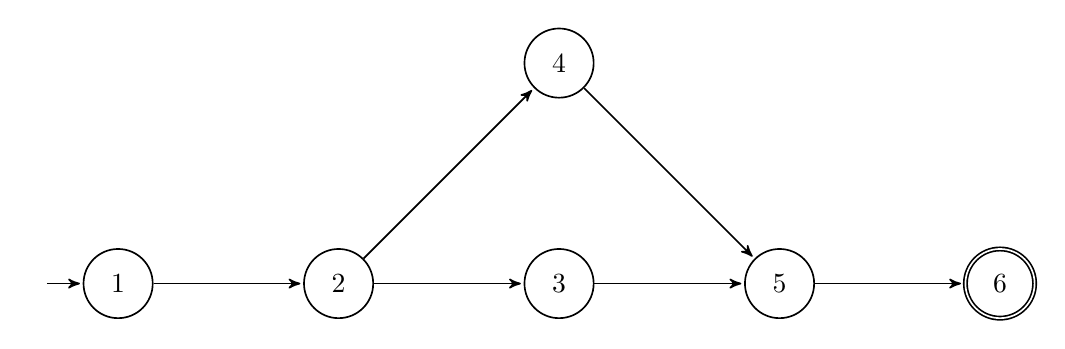
\begin{tikzpicture}[->,>=stealth',shorten >=1pt,auto,node distance=2.8cm,
                    semithick,initial text=]

  \node[initial,state]   (1)              {$1$};
  \node[state]           (2) [right of=1] {$2$};
  \node[state]           (3) [right of=2] {$3$};
  \node[state]           (4) [above of=3] {$4$};
  \node[state]           (5) [right of=3] {$5$};
  \node[accepting,state]           (6) [right of=5] {$6$};
  
  \path (1) edge              node {} (2)
        (2) edge              node {} (3)
            edge              node {} (4)
        (3) edge              node {} (5)
        (4) edge              node {} (5)
        (5) edge              node {} (6);
\end{tikzpicture}
\end{center}

\begin{itemize}
\item {\sf nodes:}
\item {\sf edges:}
\item {\sf paths of length 2: }
\end{itemize}

\end{document}
